\chapter{Testing}\label{ch:testing}

In this chapter, the different parts of the systems have been tested following the V-model \cref{ch:methodology_approach}. In the following sections, the different tests are described and the results are presented.

\section{Individual Testing}\label{sec:individual_testing}

In this section, the components are tested individually to ensure that they are working as expected, that is the drone, the reconnaissance platform, and the communication system.

\subsection{Drone Testing}\label{subsec:drone_testing}

In order to test the drone, first static tests where taken and all the electronics was tested individually. For the motors, the ESCs and the flight controller, the first thing is to calibrate them and adjust all ports. This is done through the ArduPilot program \autocite{ardupilotMissionPlanner}. After the configuration is done, the tests are done without propellers as it can be a safety hazard to do the tests with them on, refer to \cref{fig:drone_testing}. Also it is worth noting than whenever the drone is being manipulated, the battery must be disconnected to avoid any unexpected situations.

\begin{figure}
	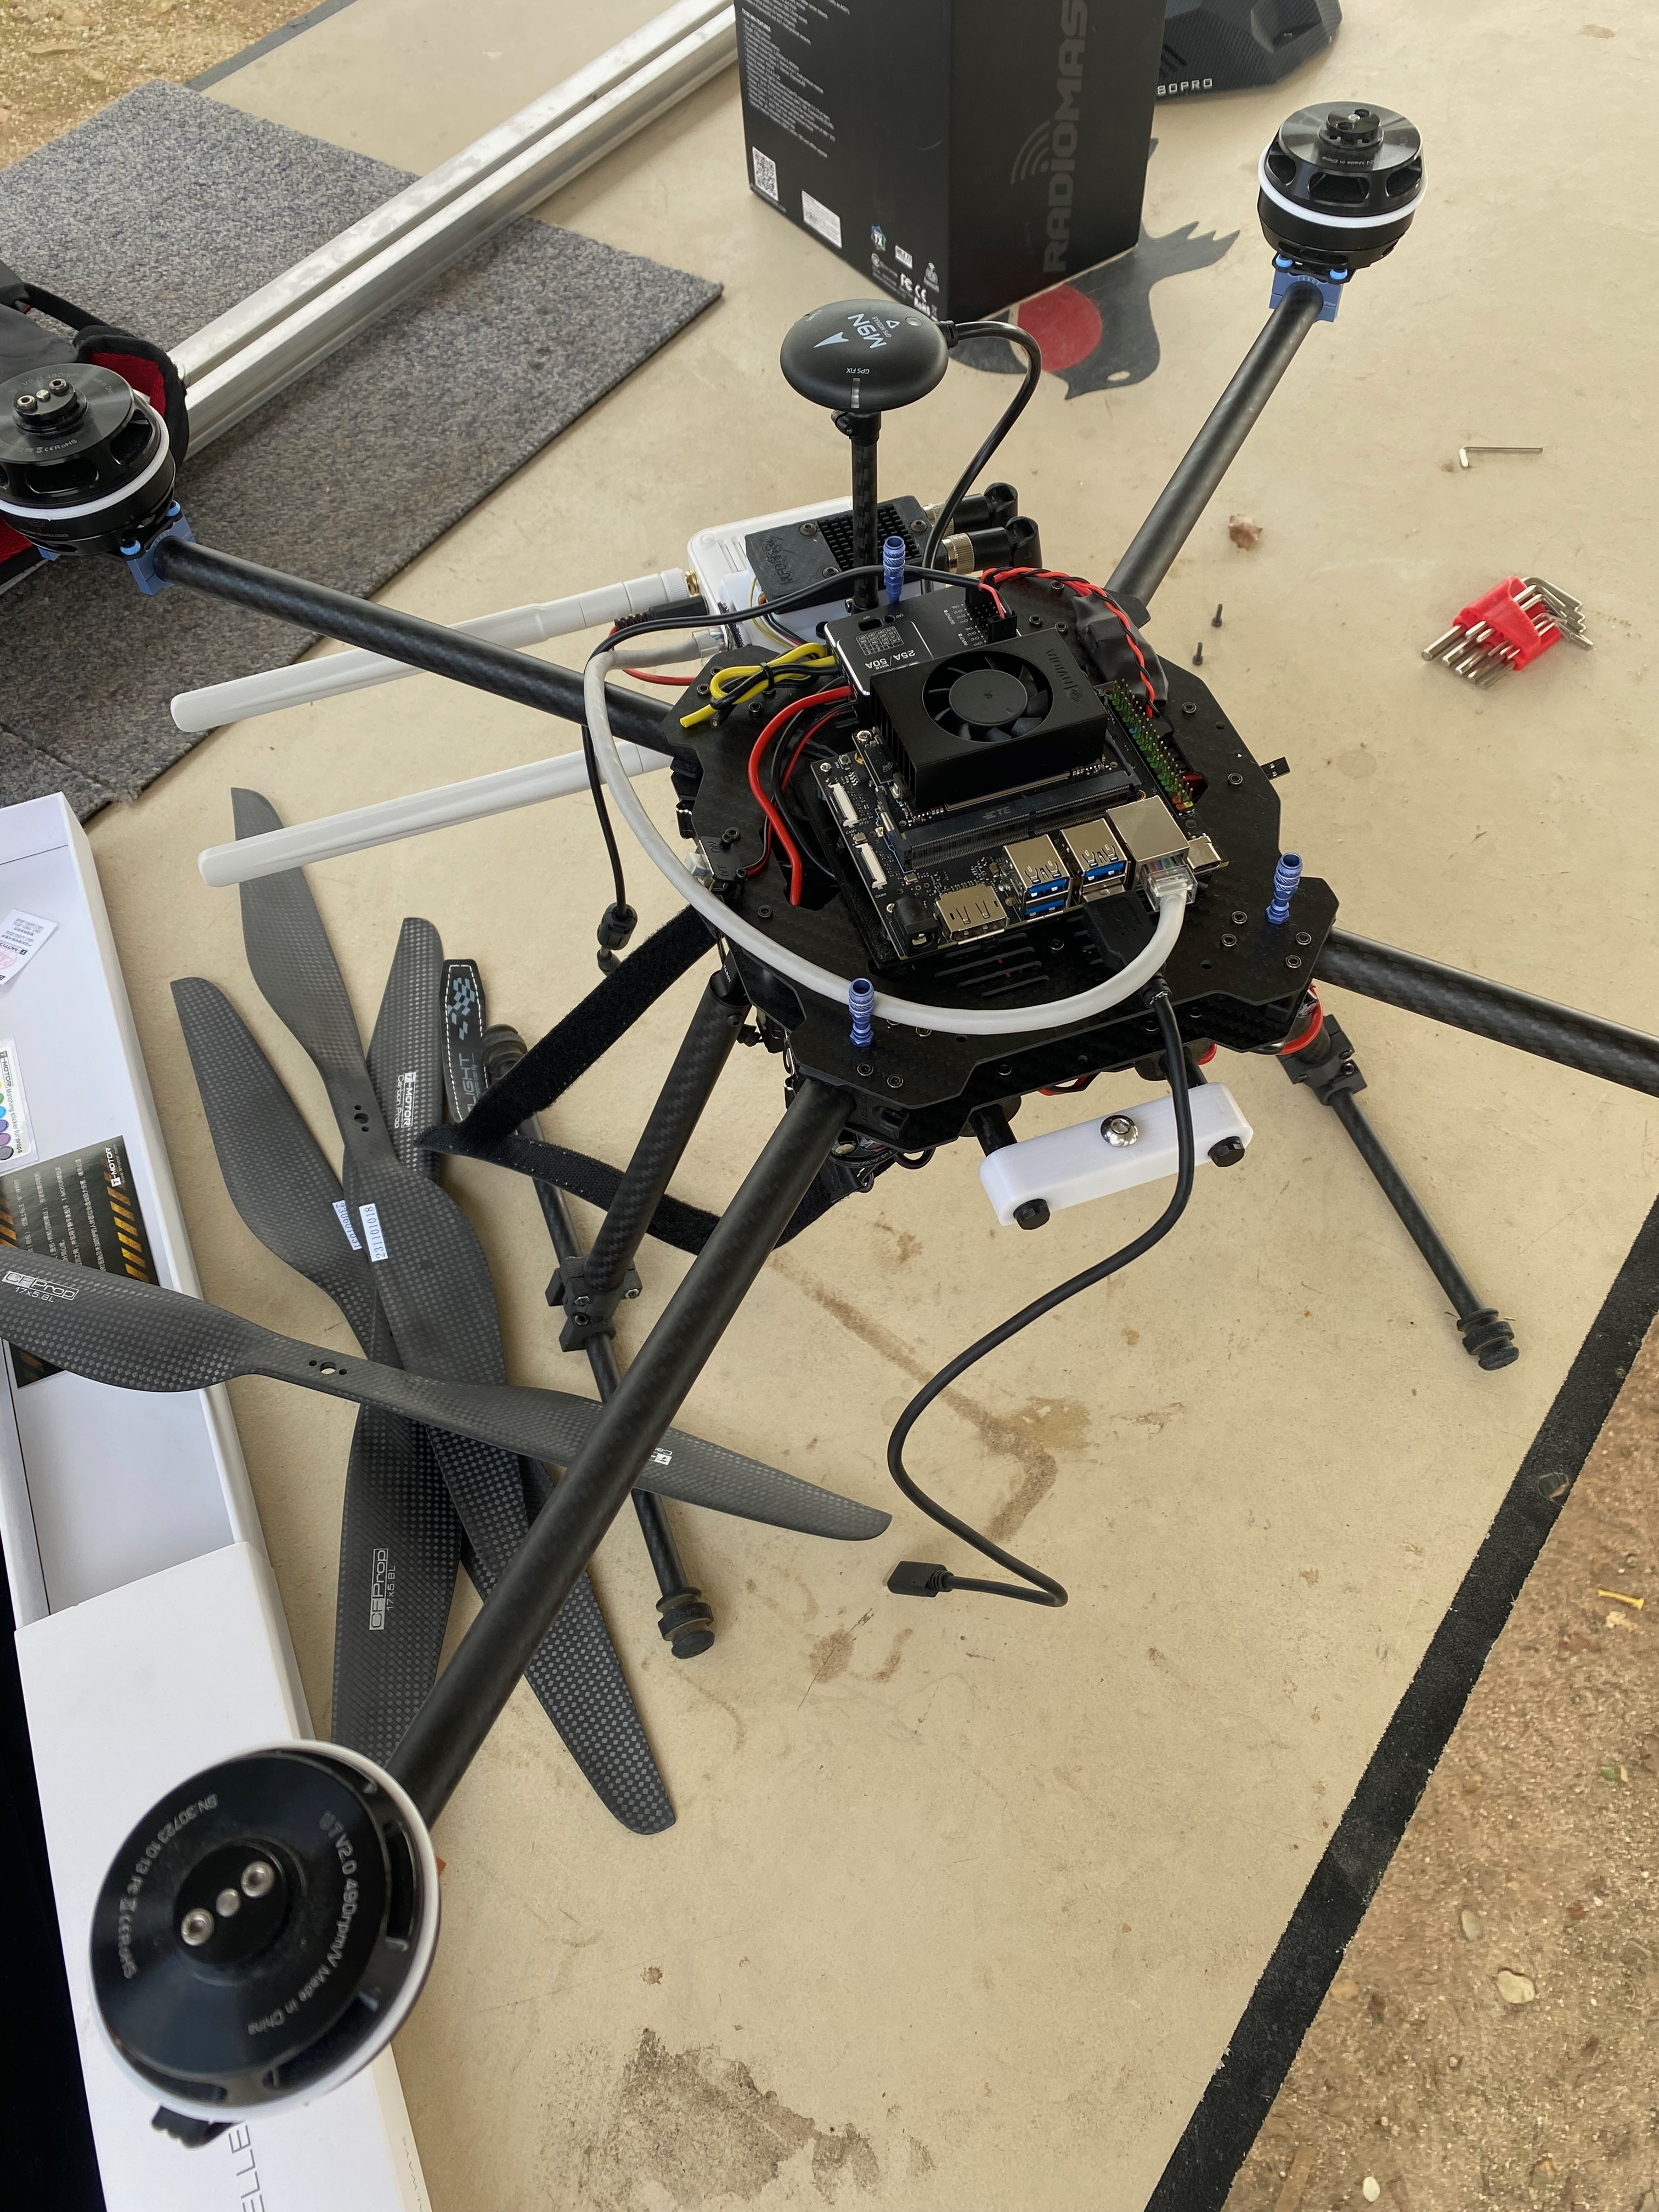
\includegraphics{testing_drone.jpeg}
	\caption{Drone testing without propellers}\label{fig:drone_testing}
\end{figure}

Once the drone is fully working statically, then the next step is to configure all the sensor, \gls{gps} and \gls{imu} in this case. Once all the sensors are configured, the next step is to test them individually. The \gls{gps} is tested by checking the position in the ArduPilot program and the \gls{imu} is tested by checking the orientation in the \gls{imu} program.

\subsection{Reconnaissance Platform Testing}\label{subsec:reconnaissance_platform_testing}

For the reconnaissance platform, the first thing to do is that everything works individually. The camera is tested by connecting it to the computer and checking that the camera is working. The camera is tested by taking a picture and checking that the picture is saved in the computer. The camera is also tested by checking that the camera is working with the Jetson Nano connected, see \cref{fig:reconnaissance_platform_testing}.

\begin{figure}
	\hfill
	\begin{subfigure}{0.4\textwidth}
		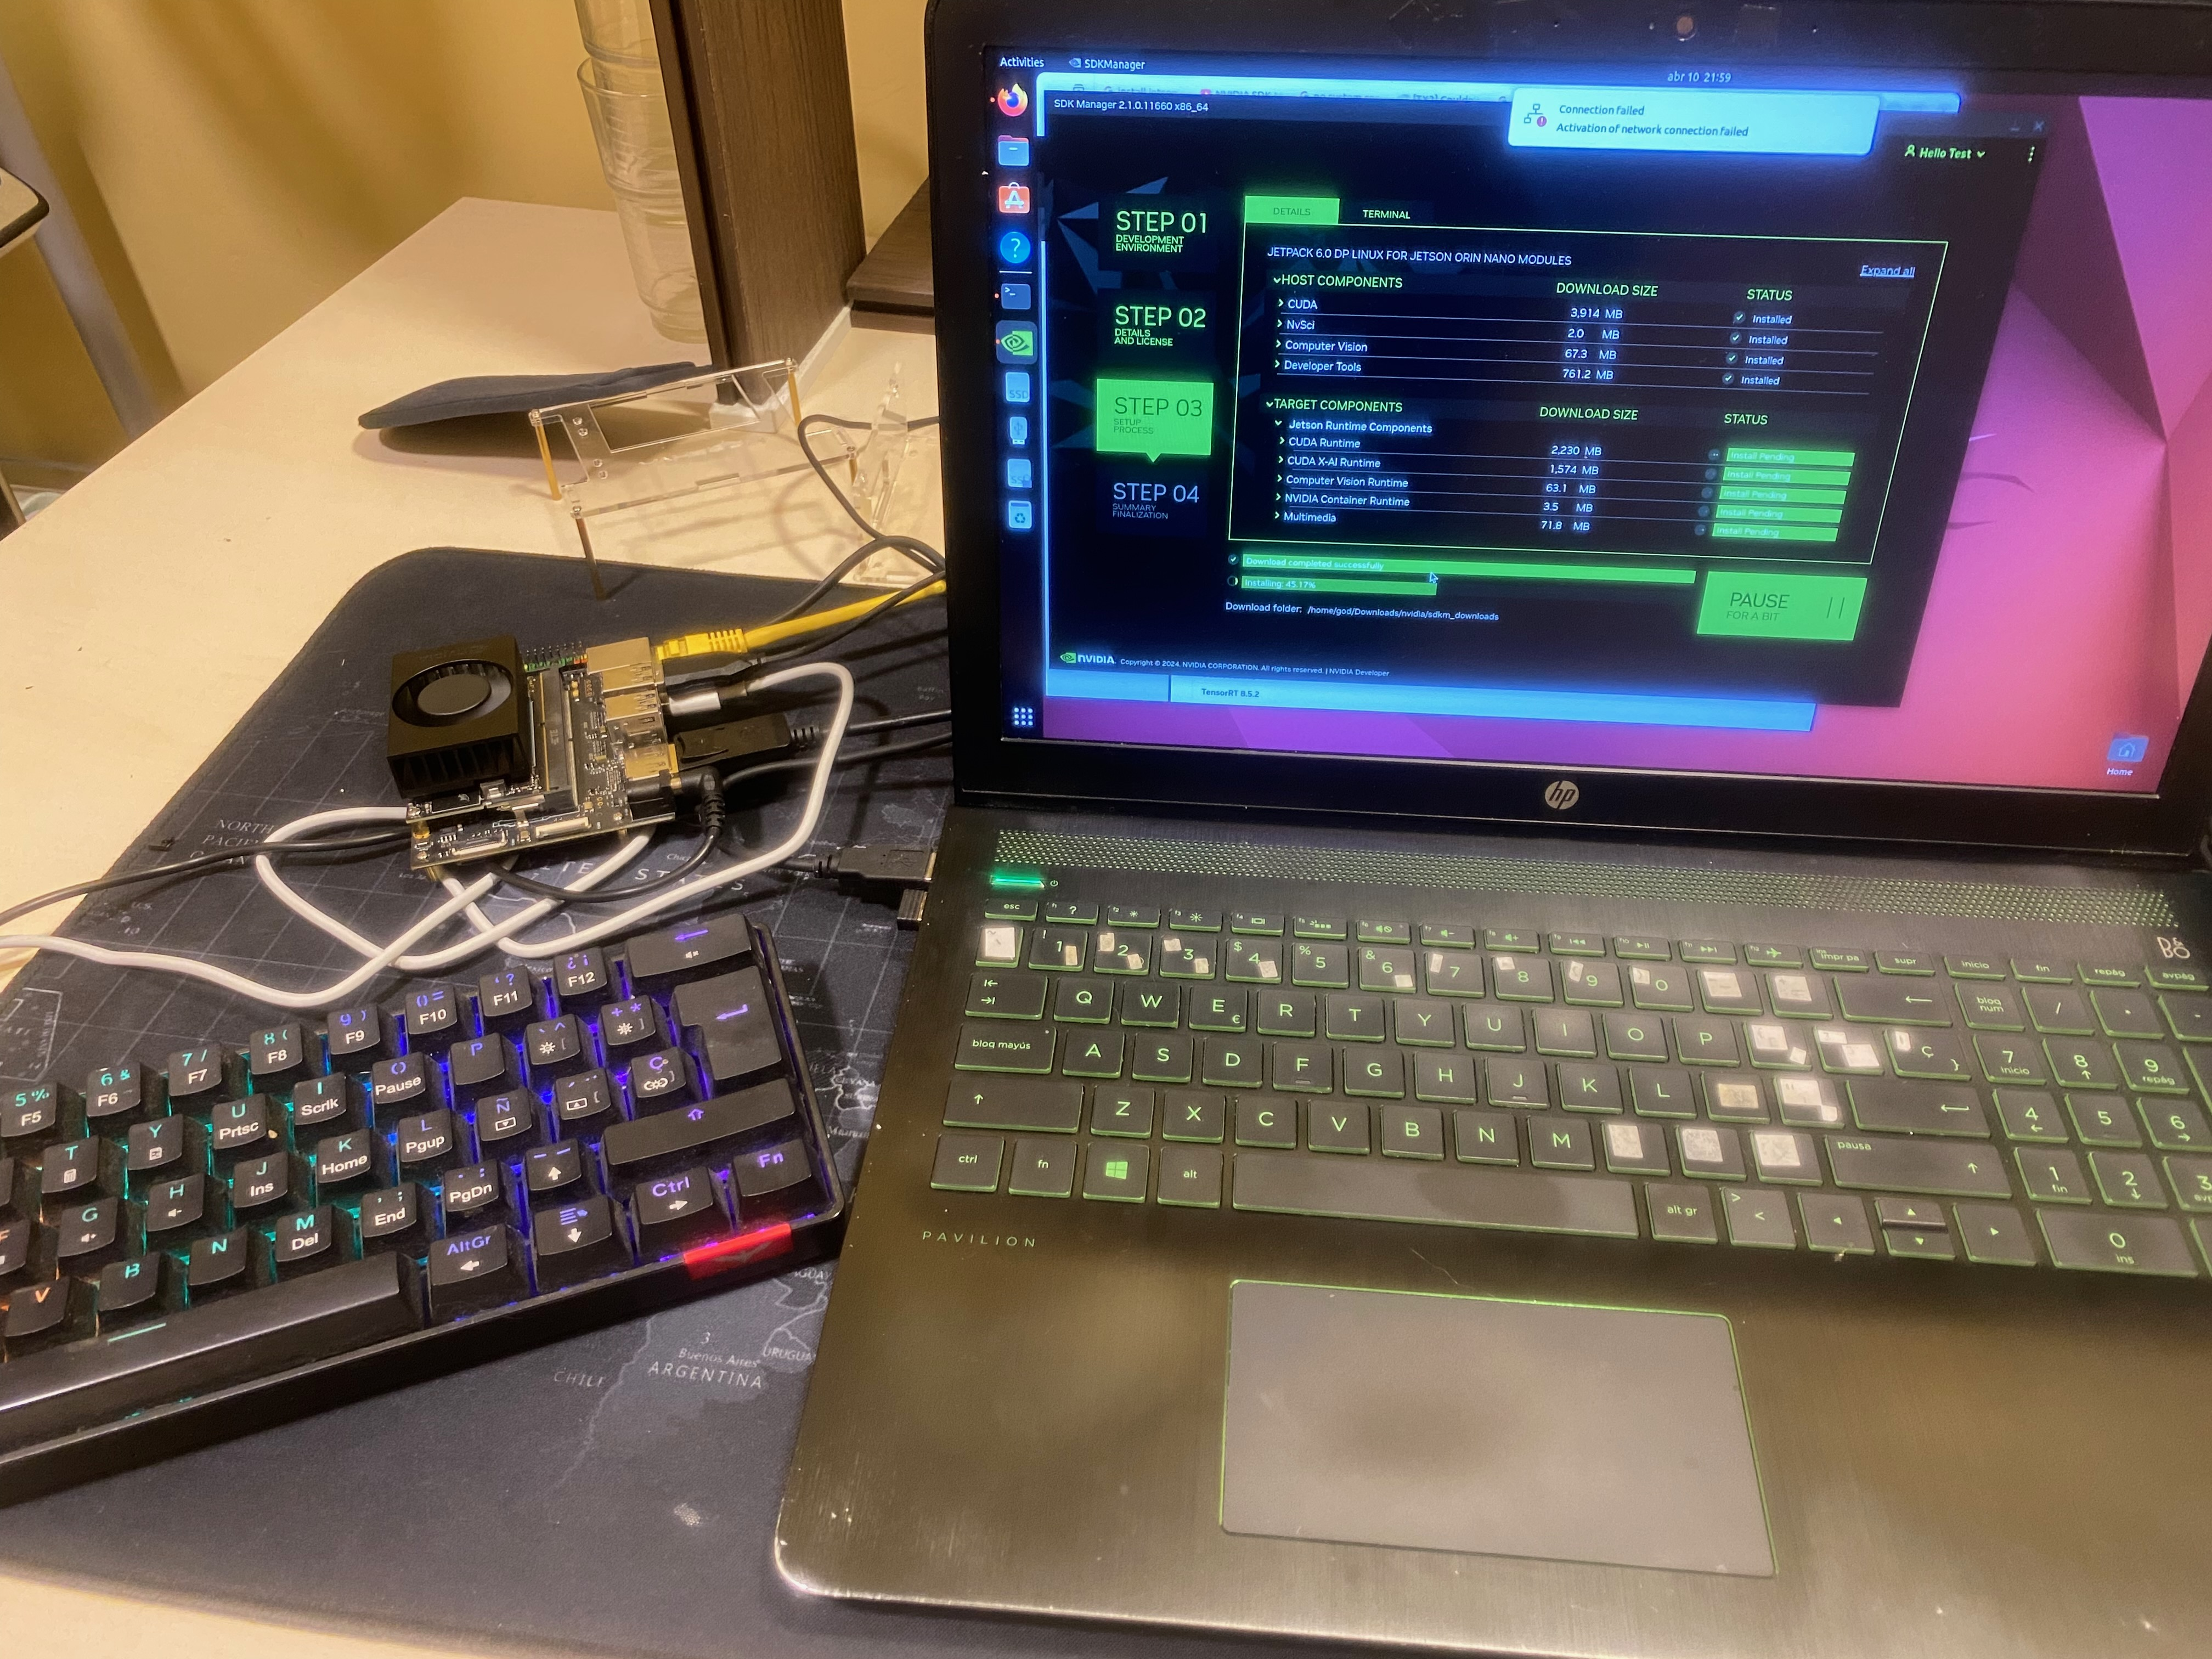
\includegraphics{testing_jetson.jpeg}
		\caption{Installation and configuration of the Jetson Nano.}\label{fig:jetson_testing}
	\end{subfigure}
	\hfill
	\begin{subfigure}{0.4\textwidth}
		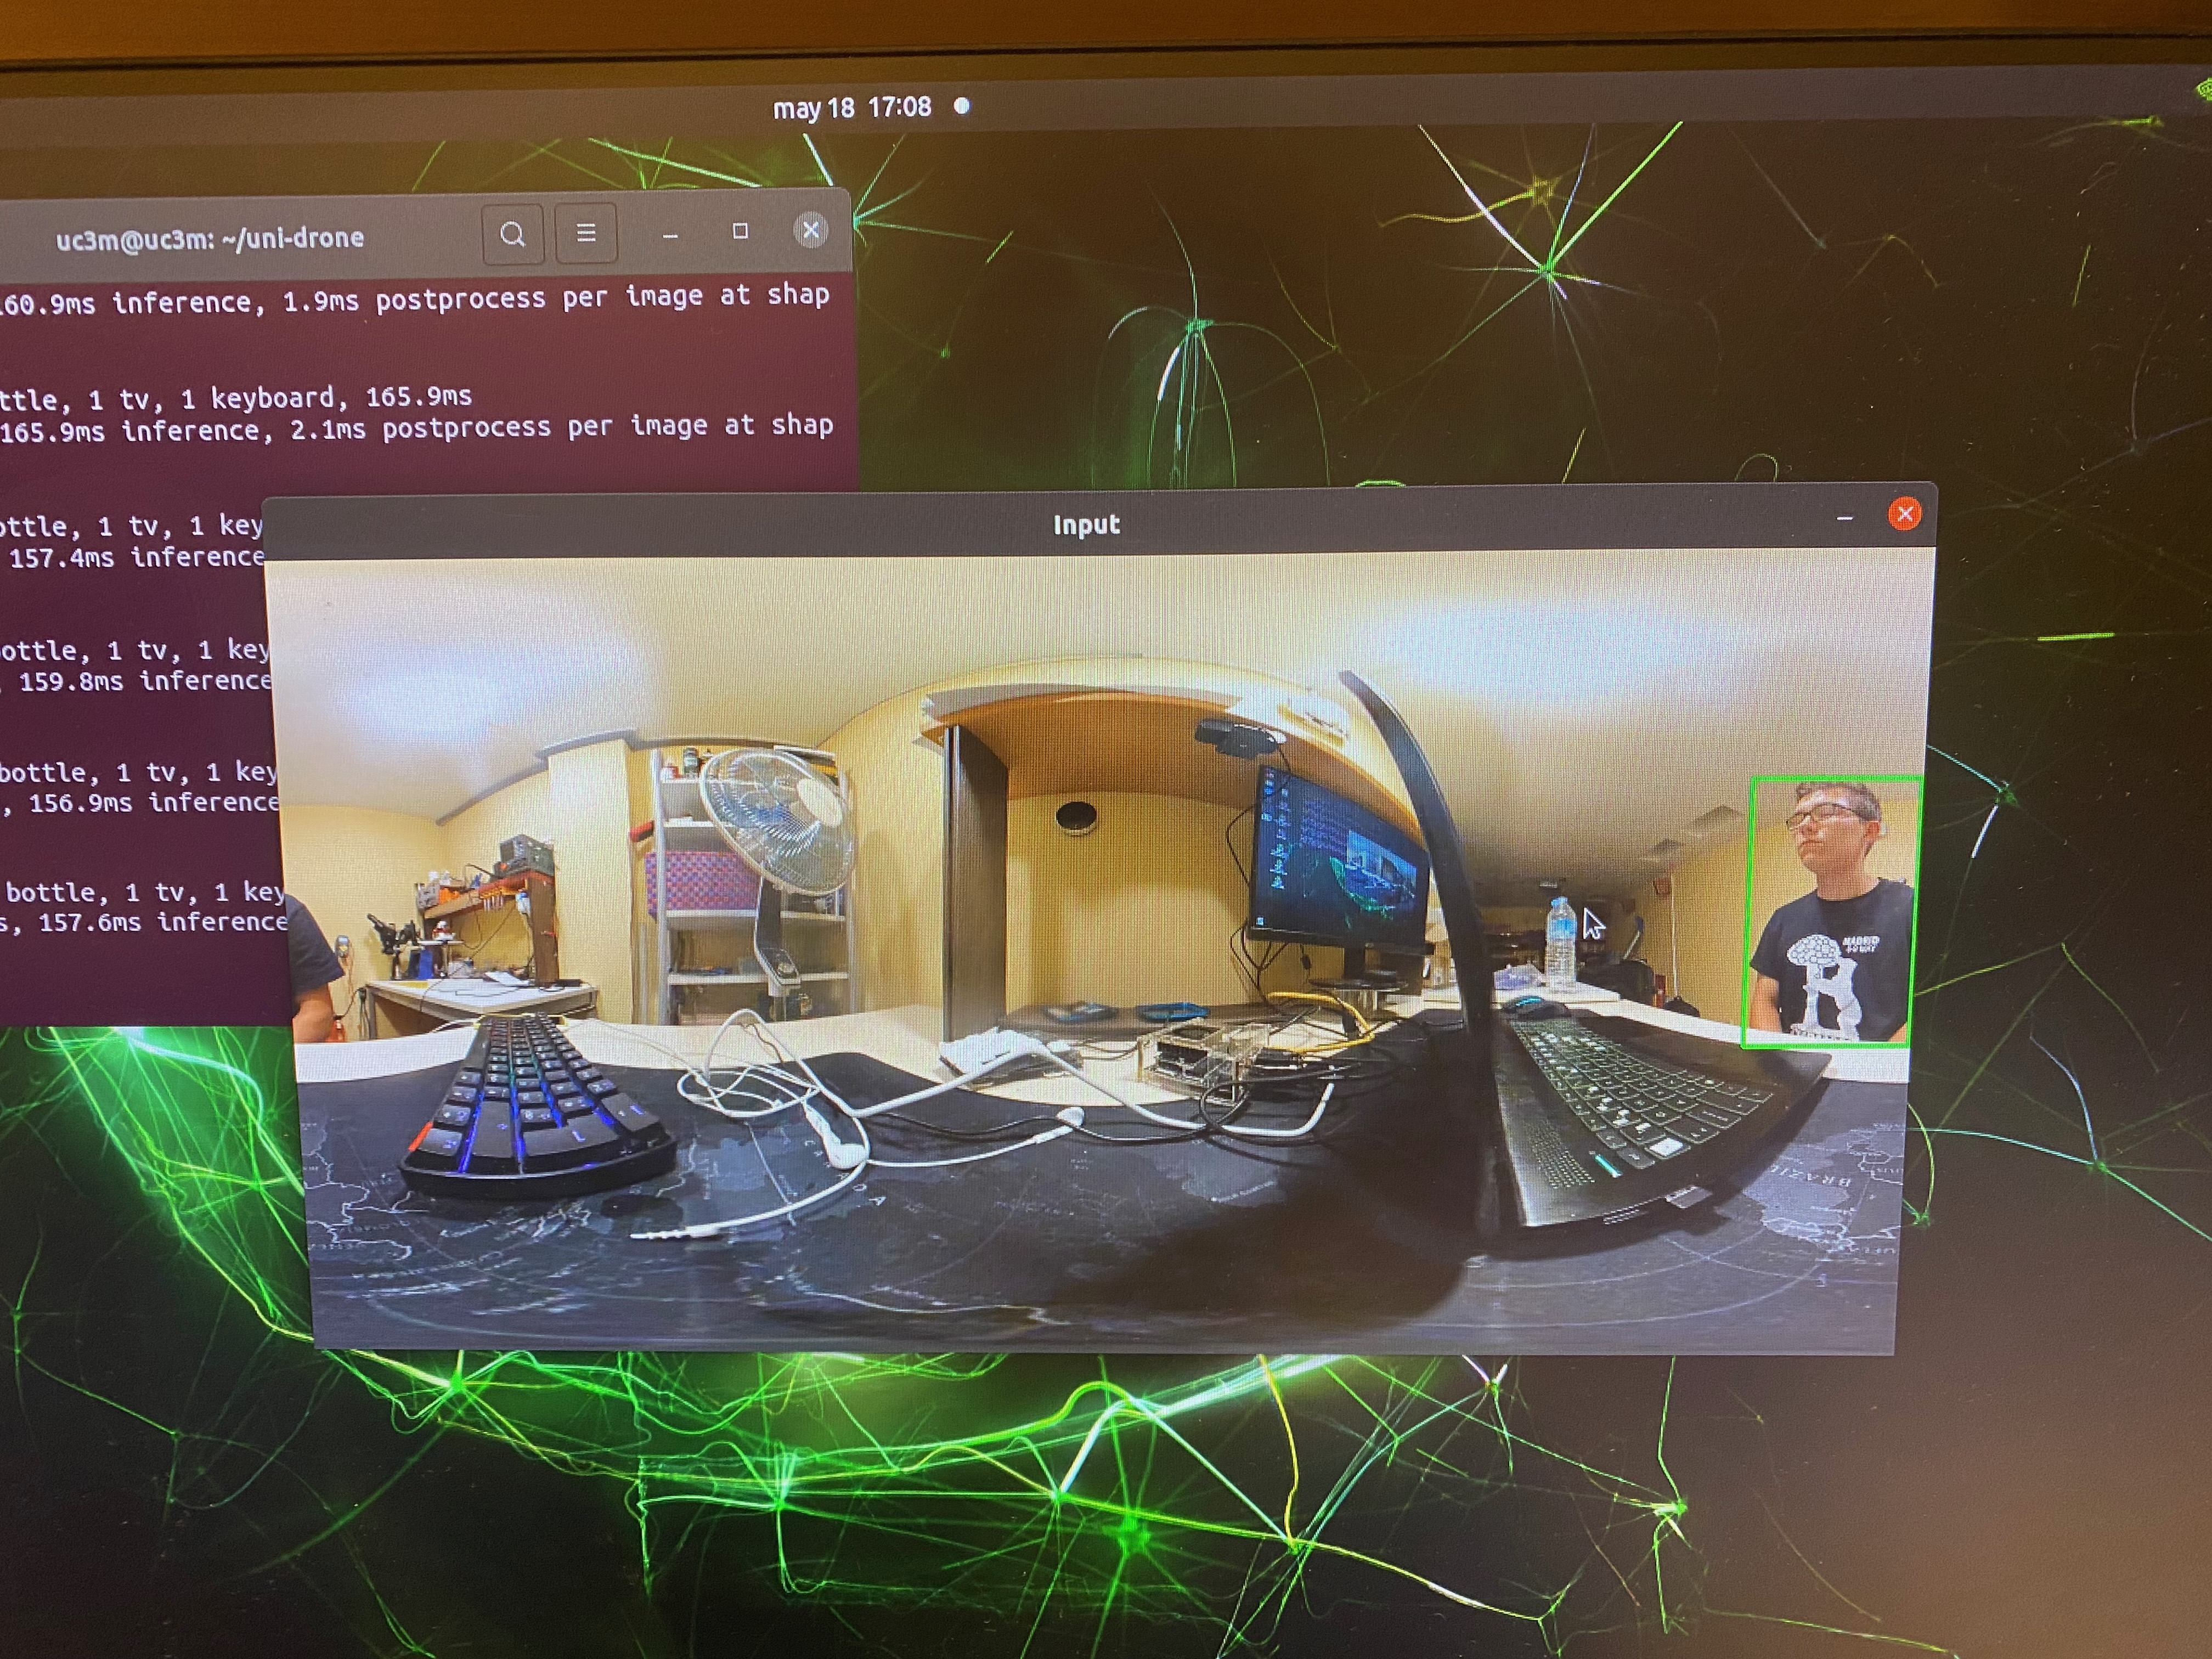
\includegraphics{testing_camera_jetson.jpeg}
		\caption{Testing the camera with the Jetson Nano.}\label{fig:jetson_camera_testing}
	\end{subfigure}
	\hfill

	\caption{Testing of the reconnaissance platform.}\label{fig:reconnaissance_platform_testing}
\end{figure}

Moreover, the server developed for the reconnaissance platform is tested by connecting the camera to the Jetson Nano and checking that the server is working. The server is tested by checking if the system is able to recognize the different objects in the image and if the system is able to send the information to the computer.

\subsection{Communication System Testing}\label{subsec:communication_system_testing}

For the communication system, the tests are done by connecting the \gls{rf} module and the \gls{4g} module to the computer and checking that the modules are working. The \gls{rf} module is tested by checking that the module is working with the computer and the \gls{4g} module is tested by checking that the module is working with the computer.

\section{General Testing}\label{sec:general_testing}

Once all the individual tests are done, the next step is to test the system as a whole. The system is tested by connecting all the components and checking that the system is working. The system is tested by checking that the drone is able to fly and that the reconnaissance platform is able to recognize the different objects in the image. The system is also tested by checking that the communication system is working and that the system is able to send the information to the computer.

For this, the drone was flown in a controlled environment in a authorized zone to comply with the regulations, see \cref{ch:regulatory_framework}. The tests were performed to test if the system was able to recongize human beings in an area of \SI{10}{\kilo\metre^2}. Moreover, all videos and images were stored in the computer and the system was able to send the information to the computer. In \cref{fig:detection_human}, an example of the system detecting a human being is shown. And also in \cref{fig:llm_detection}, the whole system working is shown and the end result of detecting and processing the images is performed.

\begin{figure}
	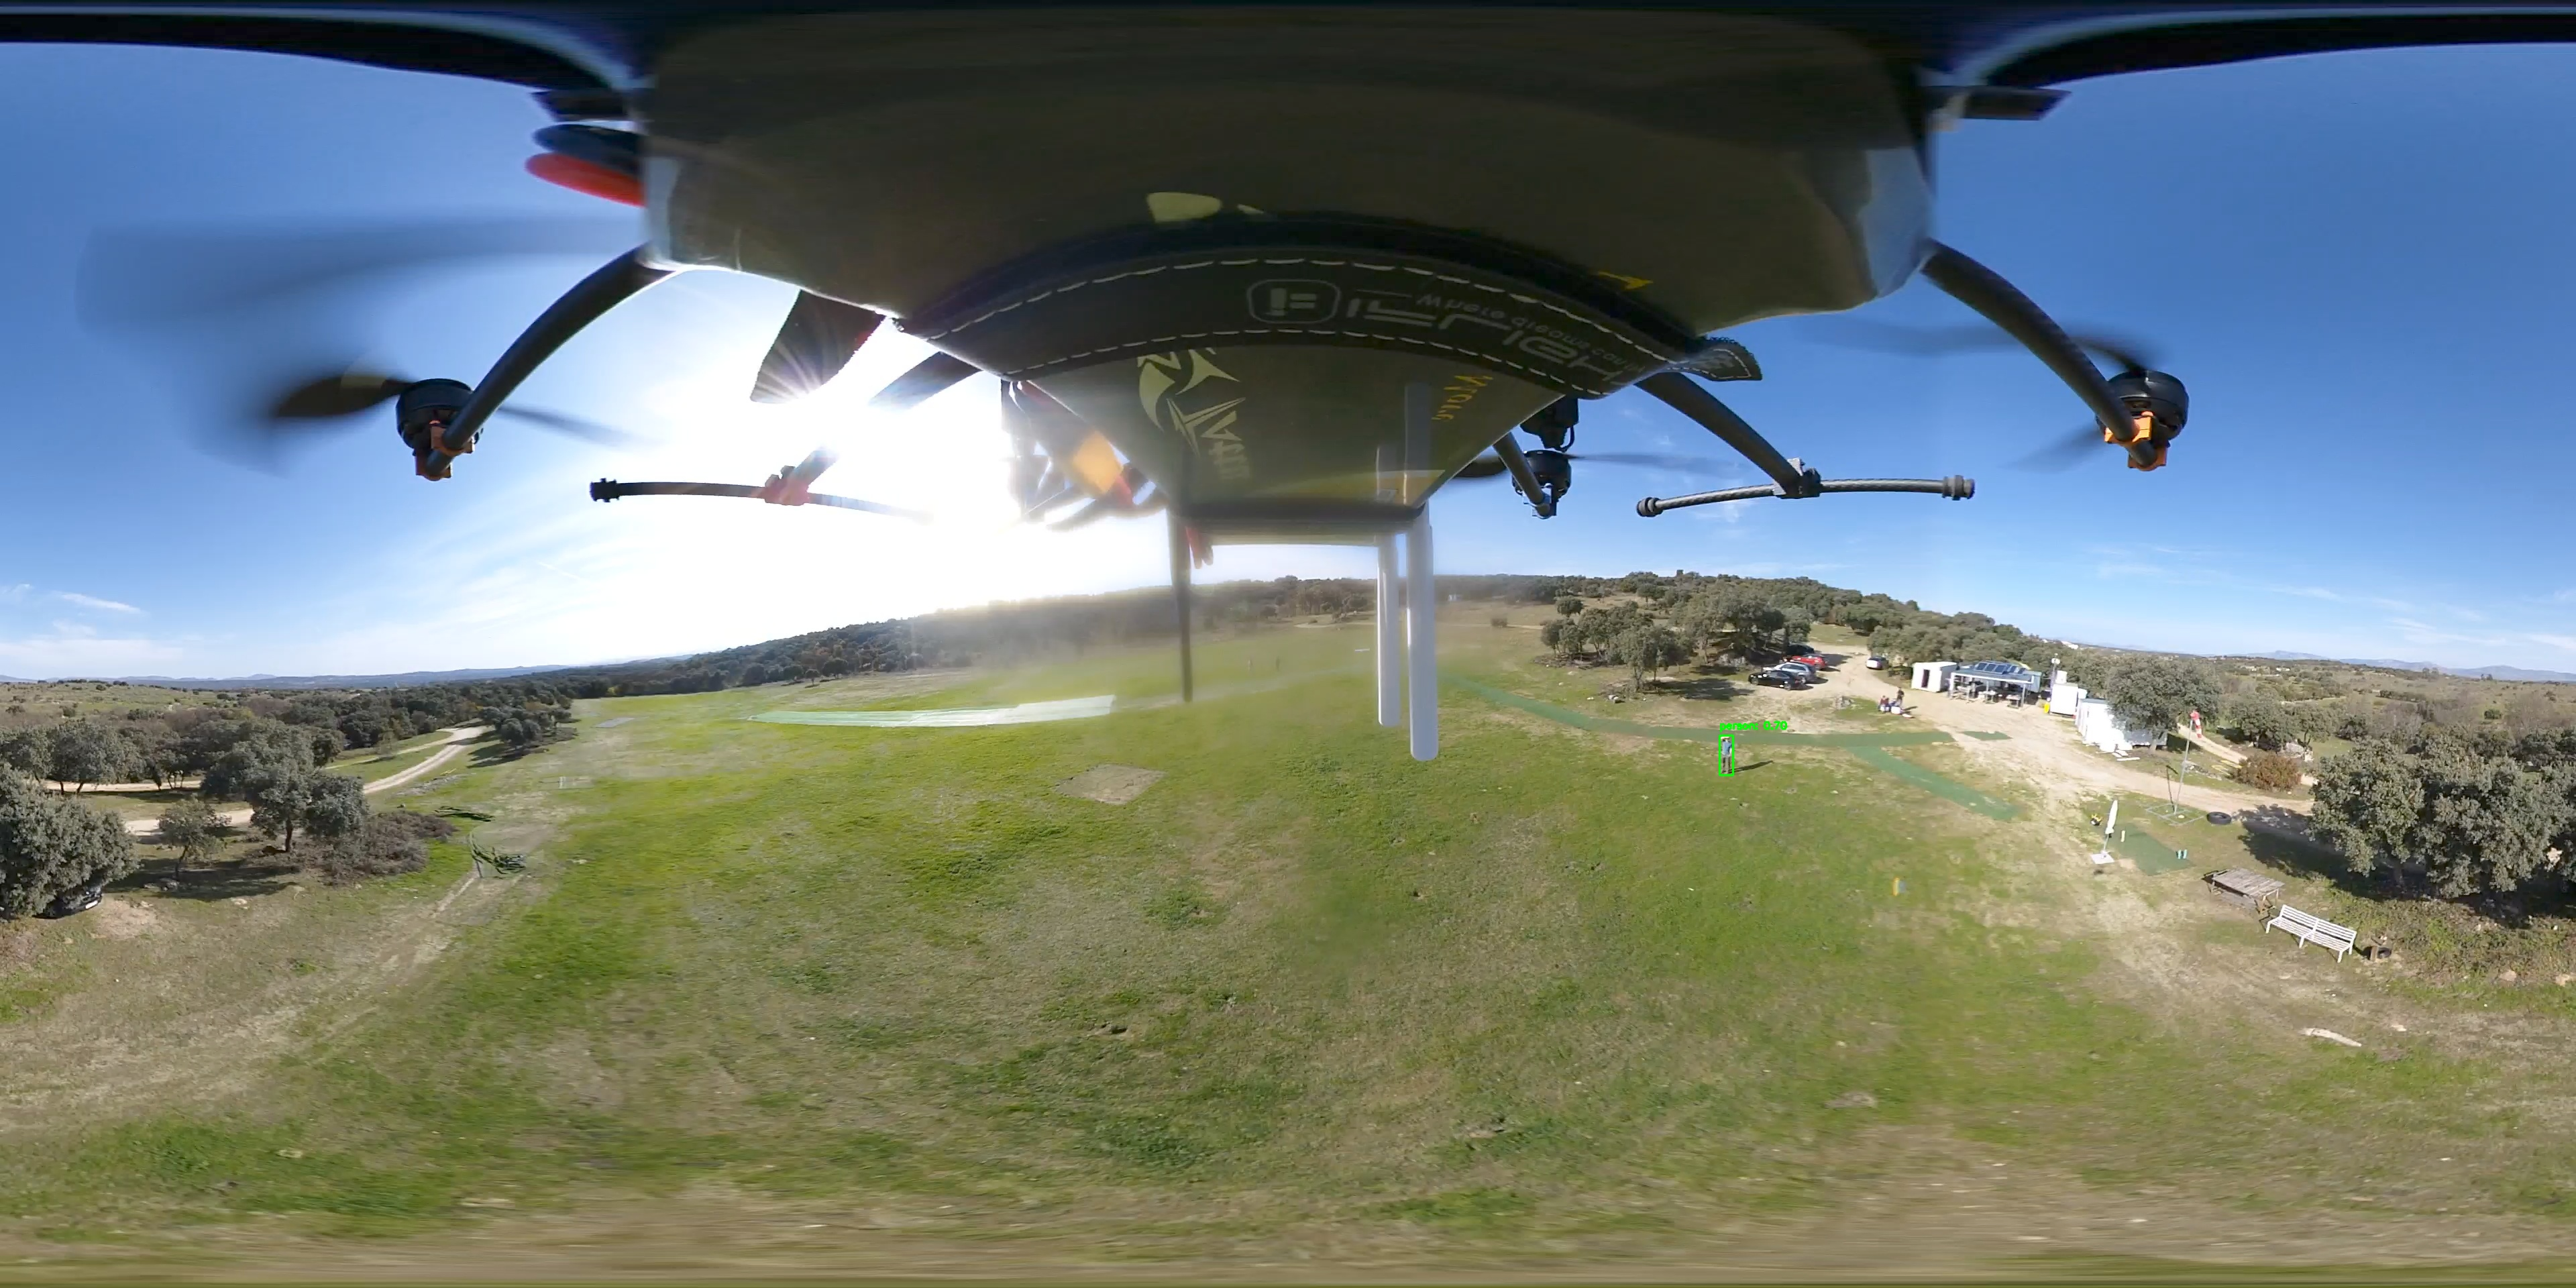
\includegraphics{detection_human.jpg}
	\caption{Human detection during the tests}\label{fig:detection_human}
\end{figure}
